% !TEX root = ./final_report.tex

\begin{figure}
        \centering
        \begin{subfigure}[b]{0.3\textwidth}
                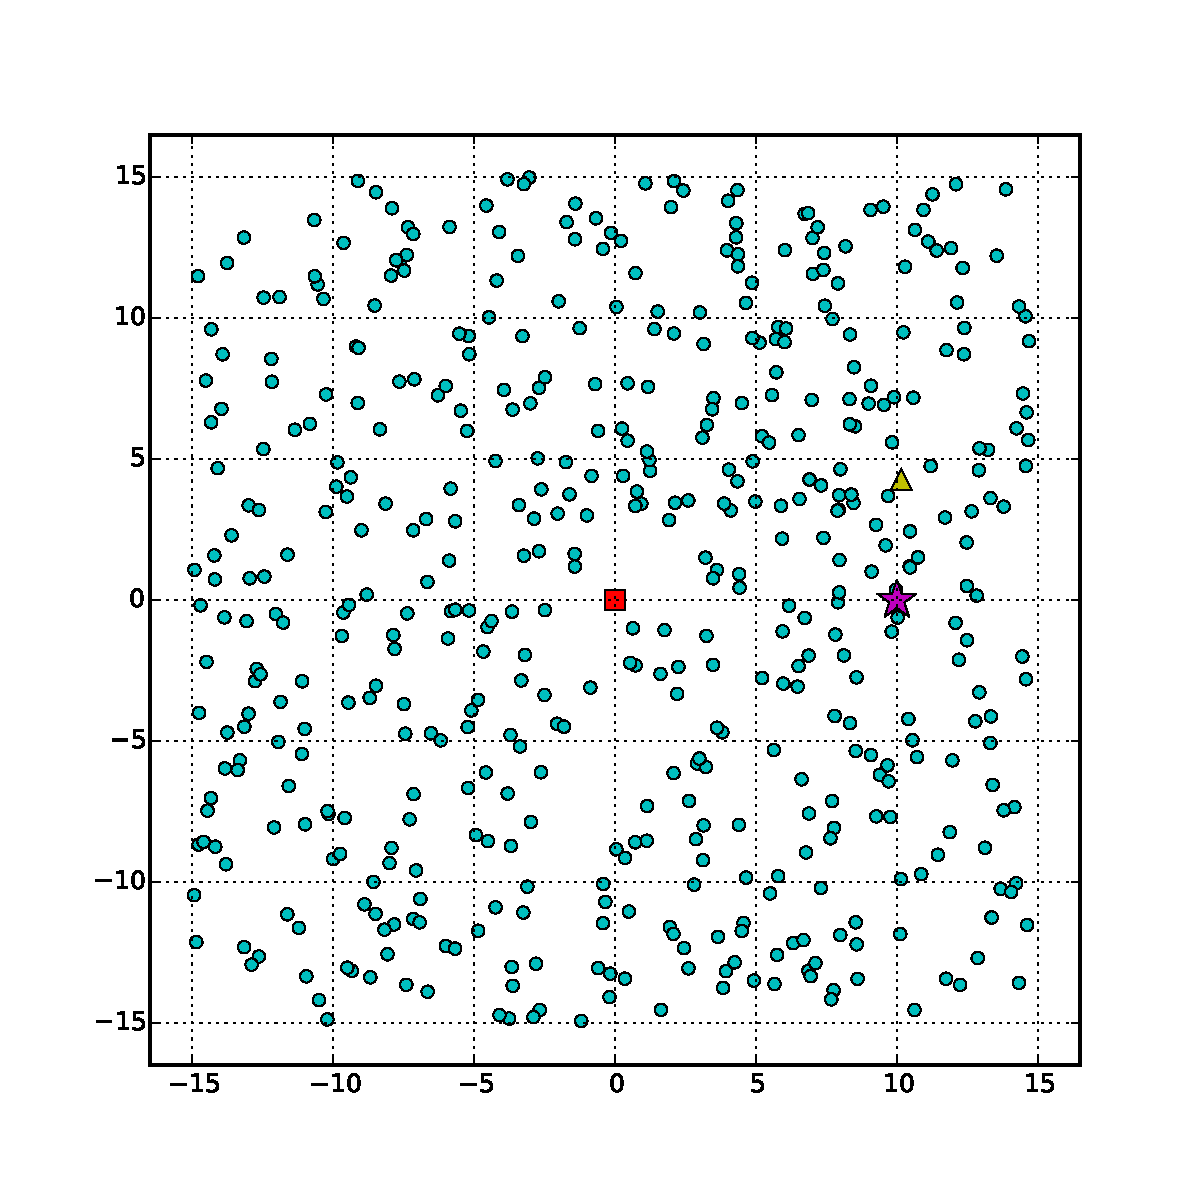
\includegraphics[width=\textwidth]{beam_bad_heading_initial}
                \caption{Initial belief state}
                \label{fig:beam_bad_heading_init}
        \end{subfigure}%
        ~ %add desired spacing between images, e. g. ~, \quad, \qquad, \hfill etc.
          %(or a blank line to force the subfigure onto a new line)
        \begin{subfigure}[b]{0.3\textwidth}
                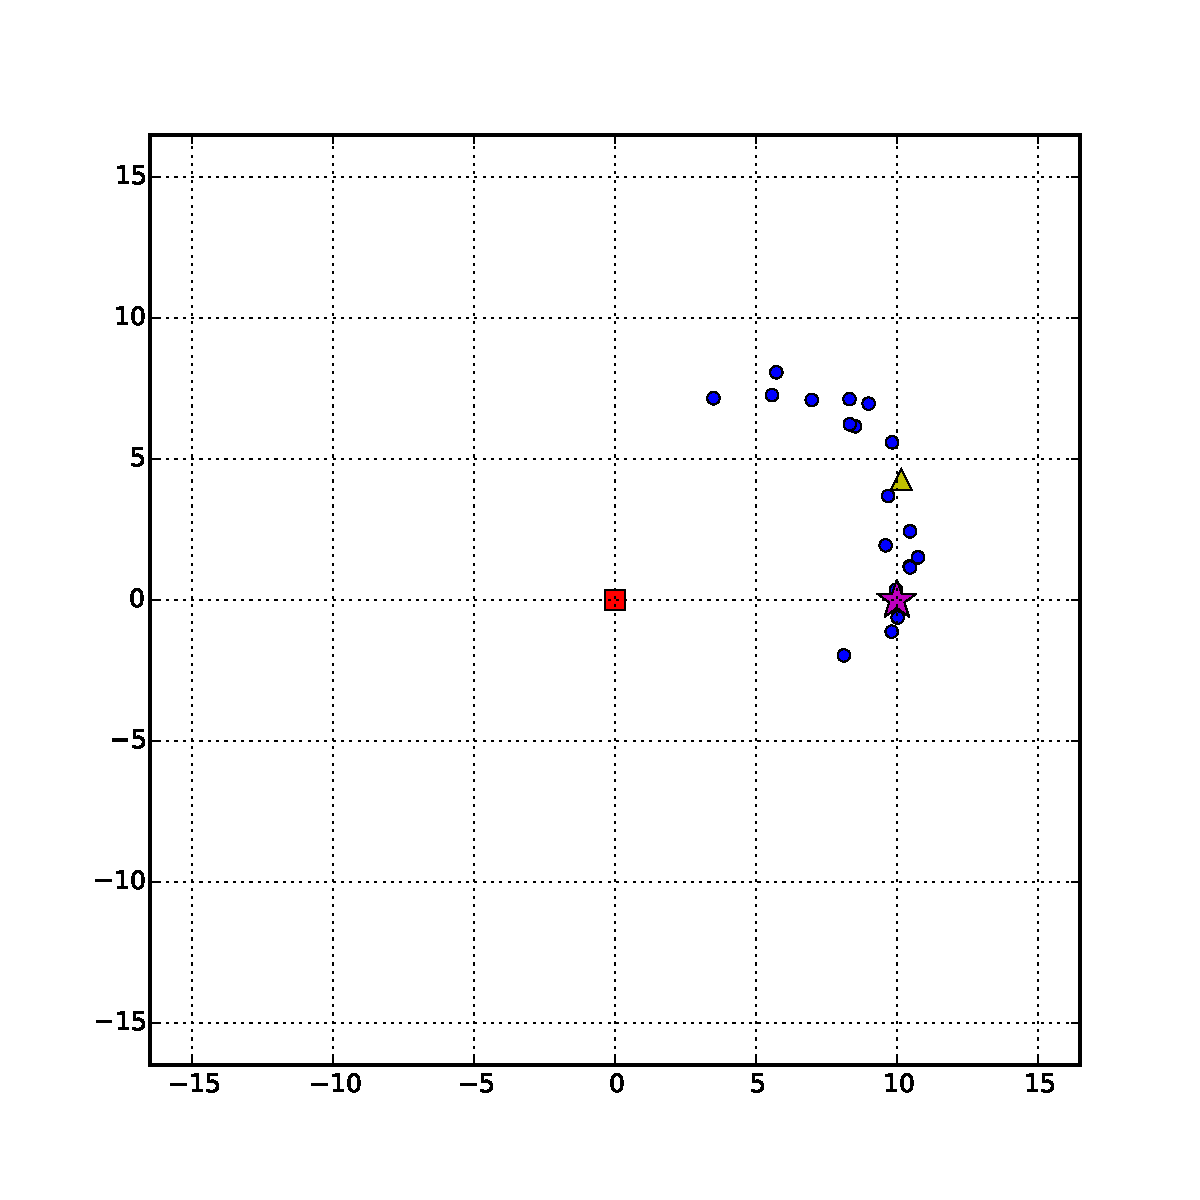
\includegraphics[width=\textwidth]{beam_bad_heading_first_obs}
                \caption{A t=0, first observation}
                \label{fig:beam_bad_heading_t_0}
        \end{subfigure}
        ~ %add desired spacing between images, e. g. ~, \quad, \qquad, \hfill etc.
          %(or a blank line to force the subfigure onto a new line)
        \begin{subfigure}[b]{0.3\textwidth}
                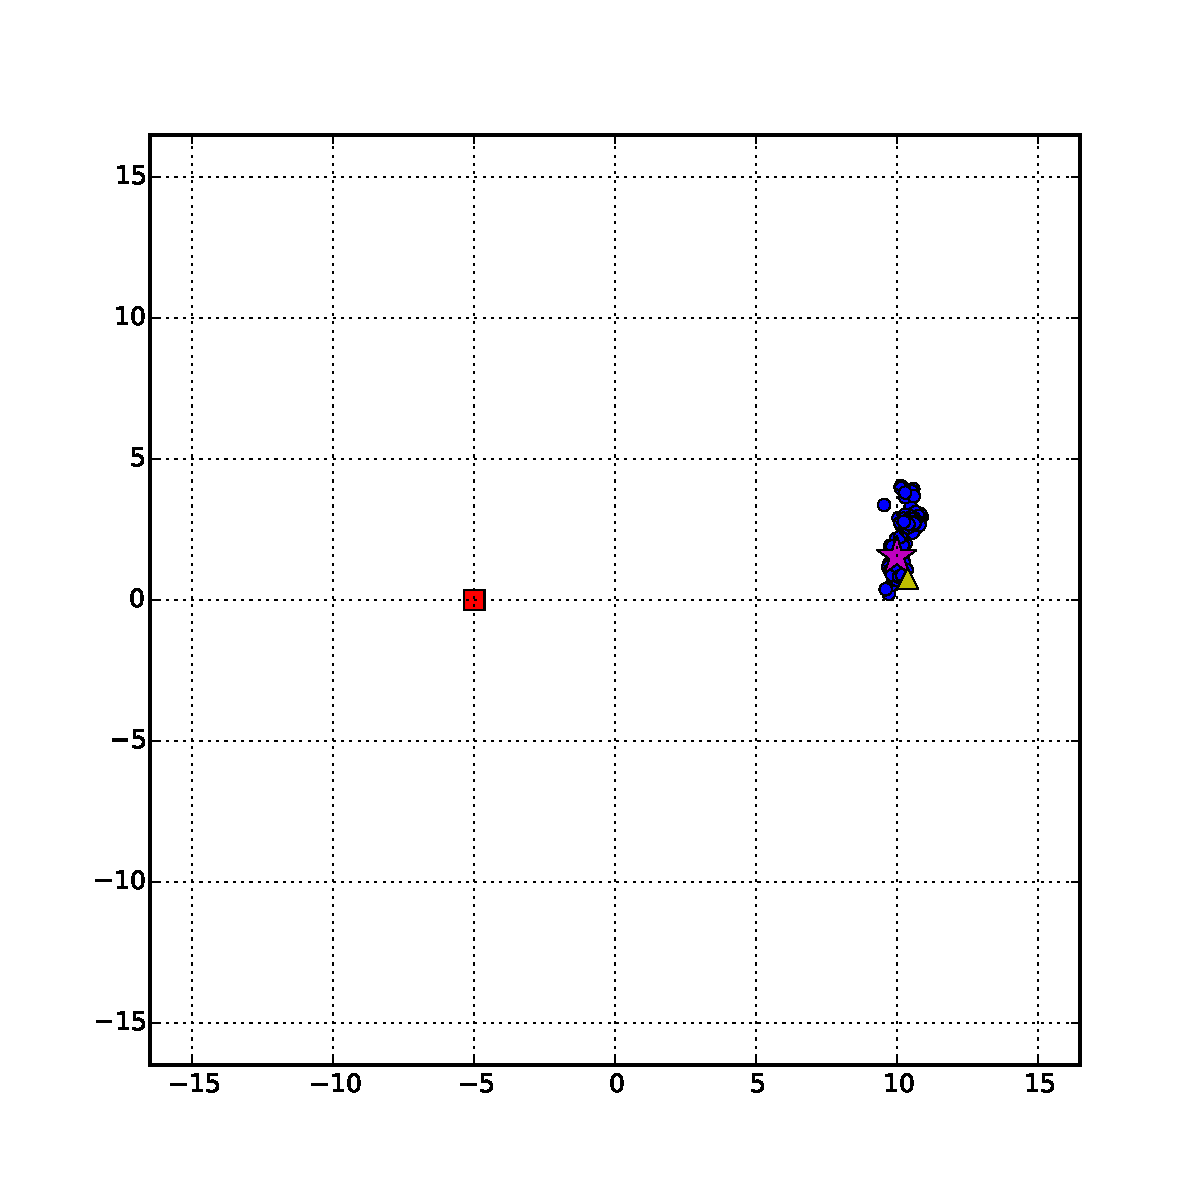
\includegraphics[width=\textwidth]{beam_bad_heading_t_1}
                \caption{t=1}
                \label{fig:beam_bad_heading_t_1}
        \end{subfigure}
        \begin{subfigure}[b]{0.3\textwidth}
                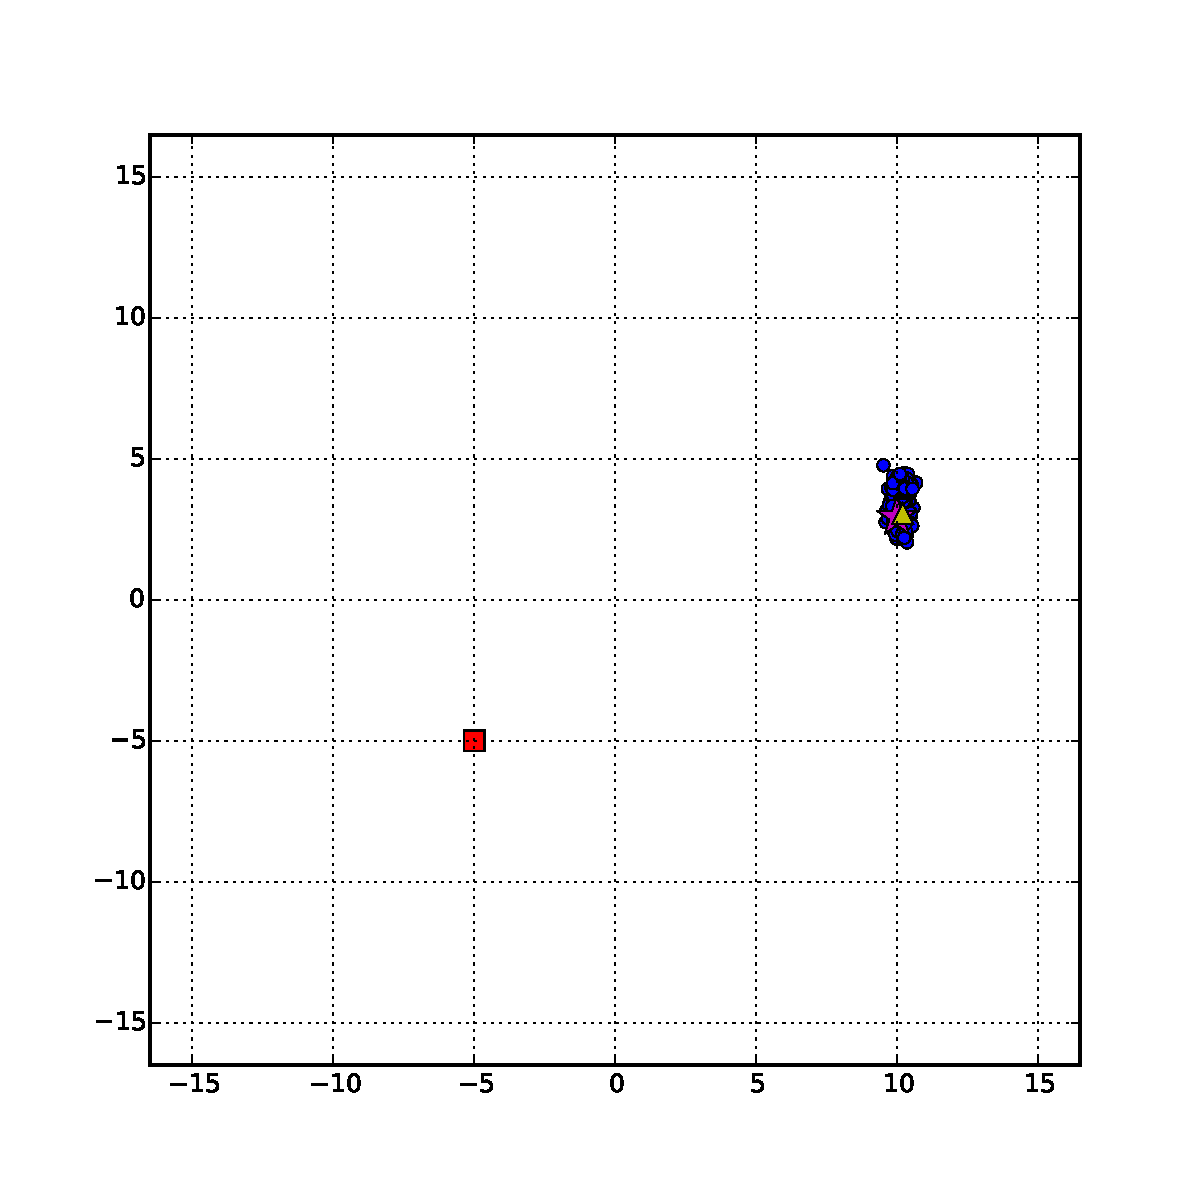
\includegraphics[width=\textwidth]{beam_bad_heading_t_2}
                \caption{t=2}
                \label{fig:beam_bad_heading_t_2}
        \end{subfigure}
        \begin{subfigure}[b]{0.3\textwidth}
                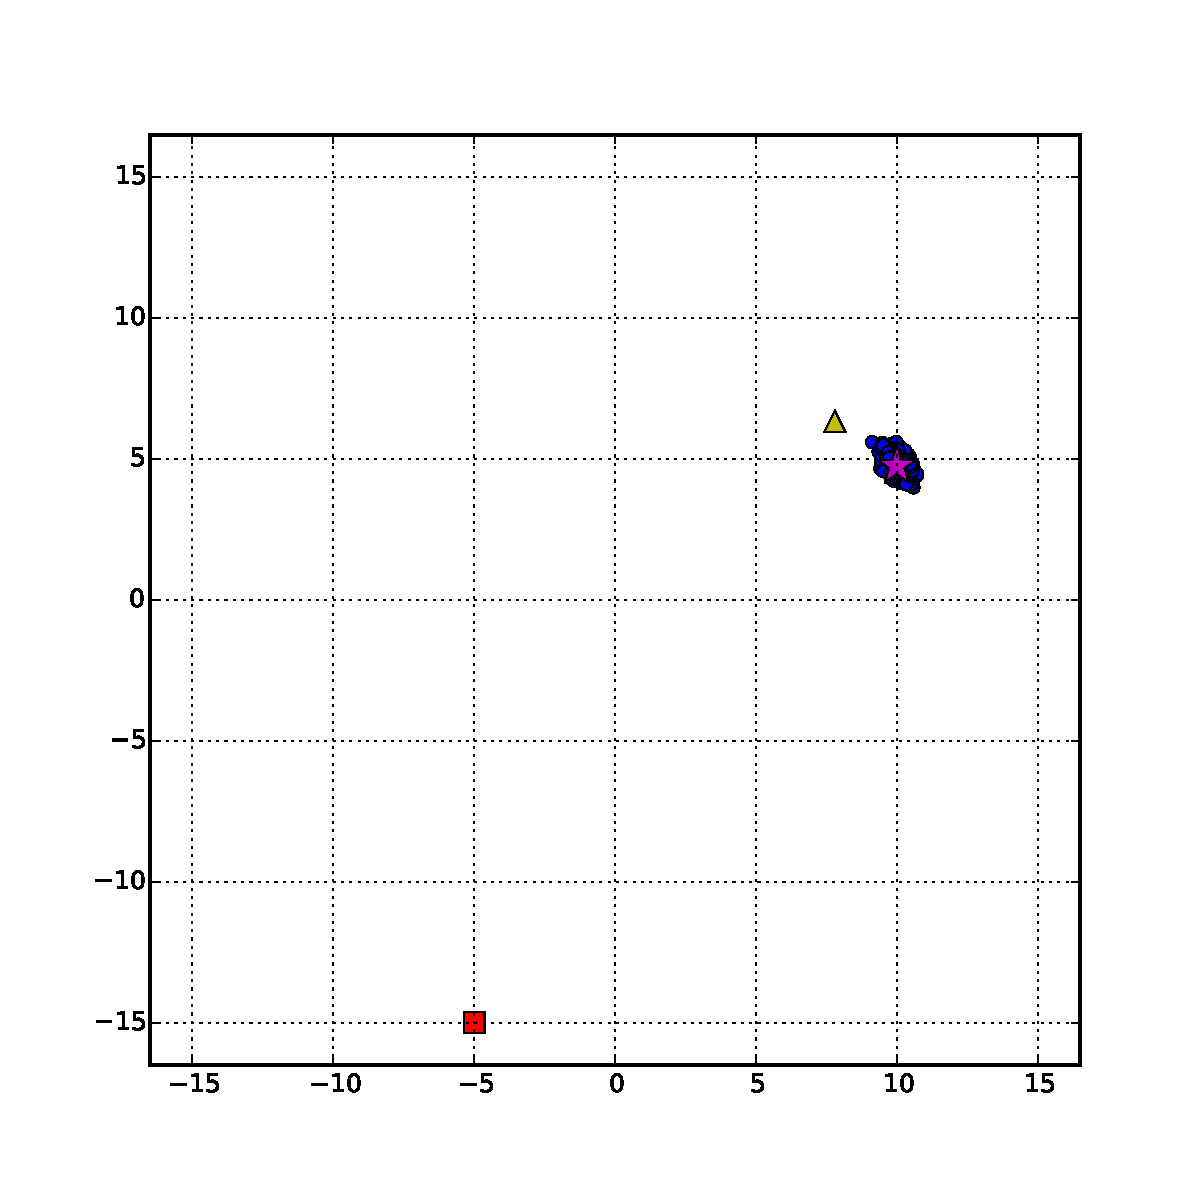
\includegraphics[width=\textwidth]{beam_bad_heading_t_4}
                \caption{t=4}
                \label{fig:beam_bad_heading_t_4}
        \end{subfigure}
        \begin{subfigure}[b]{0.3\textwidth}
                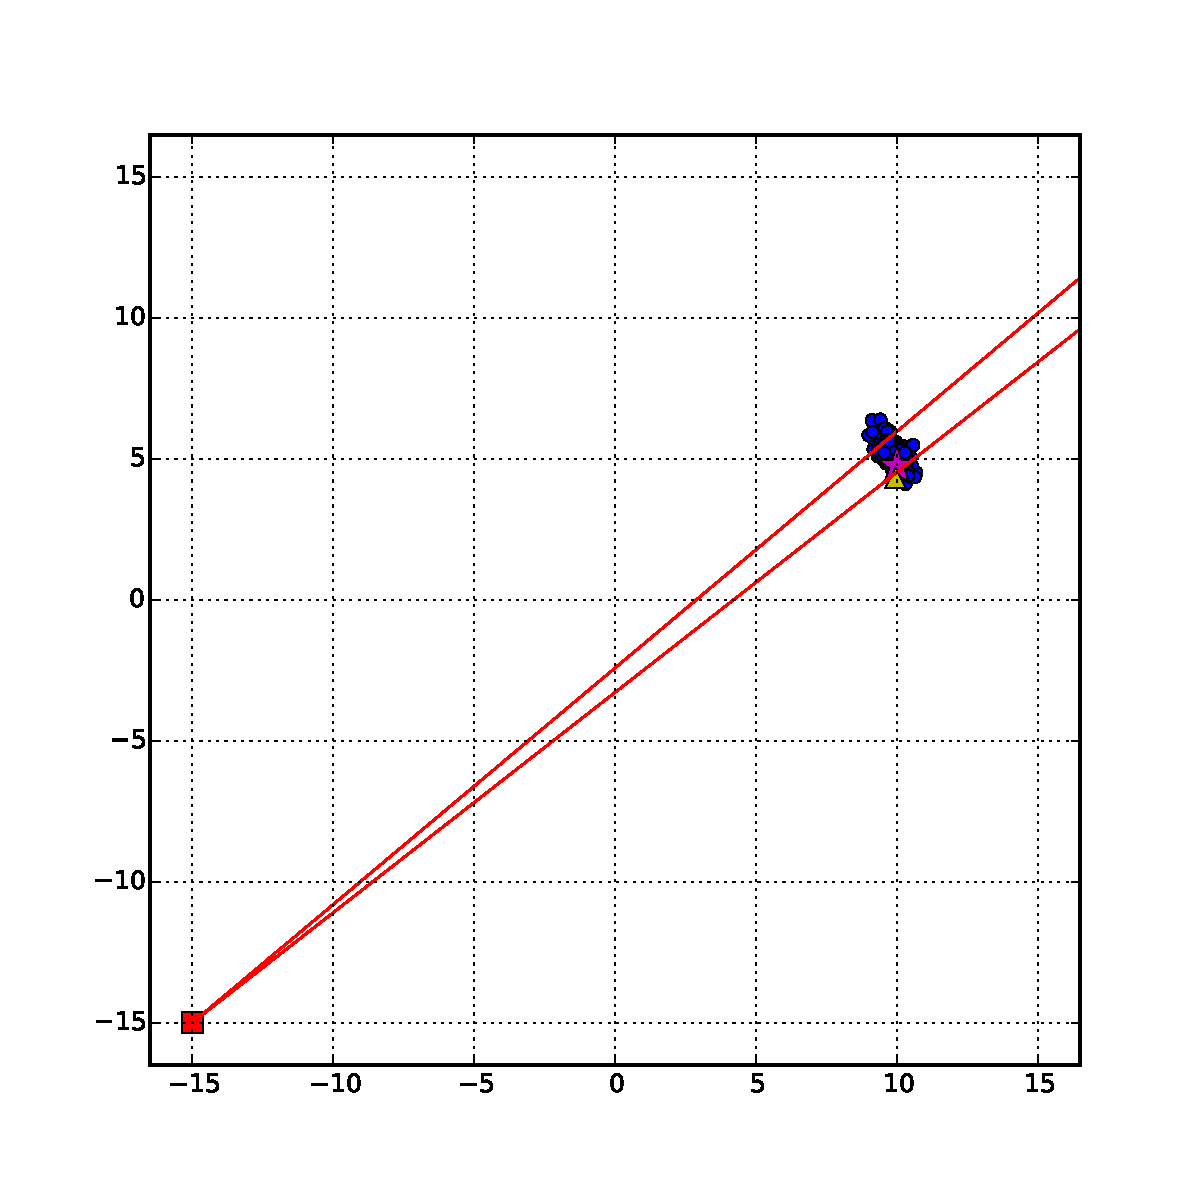
\includegraphics[width=\textwidth]{beam_bad_heading_t_6}
                \caption{t=6, agent engages target}
                \label{fig:beam_bad_heading_t_6}
        \end{subfigure}
        \caption{Progression of MC-RTBSS algorithm for the case where there is high lateral variance in the observation measurement, and the shooting mechanism is an angle target. The agent state is the red square, the current observation is the yellow triangle, the true target position is the magenta star, the belief state particles are the blue circles, and the shooting mechanism is the red beam.}\label{fig:beam_bad_heading}
\end{figure}